\documentclass[11pt]{article}

\title{PUBPOL599B Final Project}
\author{
        Emma Weaver\\
}
\date{\today}


\usepackage{Sweave}
\begin{document}
\Sconcordance{concordance:PUBPOL599B_Final_Project_Exec.tex:PUBPOL599B_Final_Project_Exec.Rnw:%
1 9 1 1 0 8 1 1 53 2 1 1 2 5 0 1 2 3 1 1 15 2 1 1 59 1 2 5 1}


\maketitle

\section{Introduction}\label{intro}
The Living Standards Measurement Study - Integrated Surveys on Agriculture (LSMS-ISA) is a household survey funded by the Gates Foundation and implemented by the World Bank. This representative panel survey is implemented in eight countries, including Tanzania. The survey has a strong focus on agriculture, but includes a variety of other household metrics including those related to Housing, Water and Sanitation, and Finance.

\section{Data analysis}\label{datas}

  The primary metric of interest is the amount a household spent on improvements to the home in the past year, beyond what was spent on repairs. It is important to understand the relationship between this metric and other, secondary metrics such as the amount spent on repairs, and the use of various mobile money platforms. The below includes summary statistics for these variables. 

% Table created by stargazer v.5.2 by Marek Hlavac, Harvard University. E-mail: hlavac at fas.harvard.edu
% Date and time: Thu, Mar 08, 2018 - 10:09:18 PM
\begin{table}[!htbp] \centering 
  \caption{Mean and Spread values} 
  \label{measures} 
\begin{tabular}{@{\extracolsep{5pt}}lccccc} 
\\[-1.8ex]\hline 
\hline \\[-1.8ex] 
Statistic & \multicolumn{1}{c}{N} & \multicolumn{1}{c}{Mean} & \multicolumn{1}{c}{St. Dev.} & \multicolumn{1}{c}{Min} & \multicolumn{1}{c}{Max} \\ 
\hline \\[-1.8ex] 
Value\_of\_Repairs & 30 & 32,670.450 & 22,564.920 & 1,402.778 & 88,579.710 \\ 
Value\_of\_Improvements & 30 & 24,231.530 & 21,831.460 & 0.000 & 82,916.670 \\ 
MPesa\_Use & 30 & 1.679 & 0.194 & 1.420 & 2.000 \\ 
Ezy\_Pesa\_Use & 30 & 1.983 & 0.039 & 1.833 & 2.000 \\ 
Airtel\_Use & 30 & 1.879 & 0.099 & 1.701 & 2.000 \\ 
\hline \\[-1.8ex] 
\end{tabular} 
\end{table}   As the table shows, households on average spend more on repairs than improvements. 
  
\section{Mapping the Data}\label{map}
  Research suggests that the use of mobile money platforms increases financial inclusion \footnote{http://siteresources.worldbank.org/EXTINFORMATIONANDCOMMUNICATIONANDTECHNOLOGIES/Resources/IC4D-2012-Chapter-4.pdf}. One question asked in the LSMS-ISA survey is whether the household has used various mobile money platforms to transfer money in the last 12 months. Given that the use of mobile money is thought to increase financial inclusion, the relationship between the use of mobile money, the amount of money spent on repairs to the home, and the amount beyond this spent on improvements could be interesting. One way to visualize this data is through mapping the data by region. 
  

\begin{figure}[h]
\centering
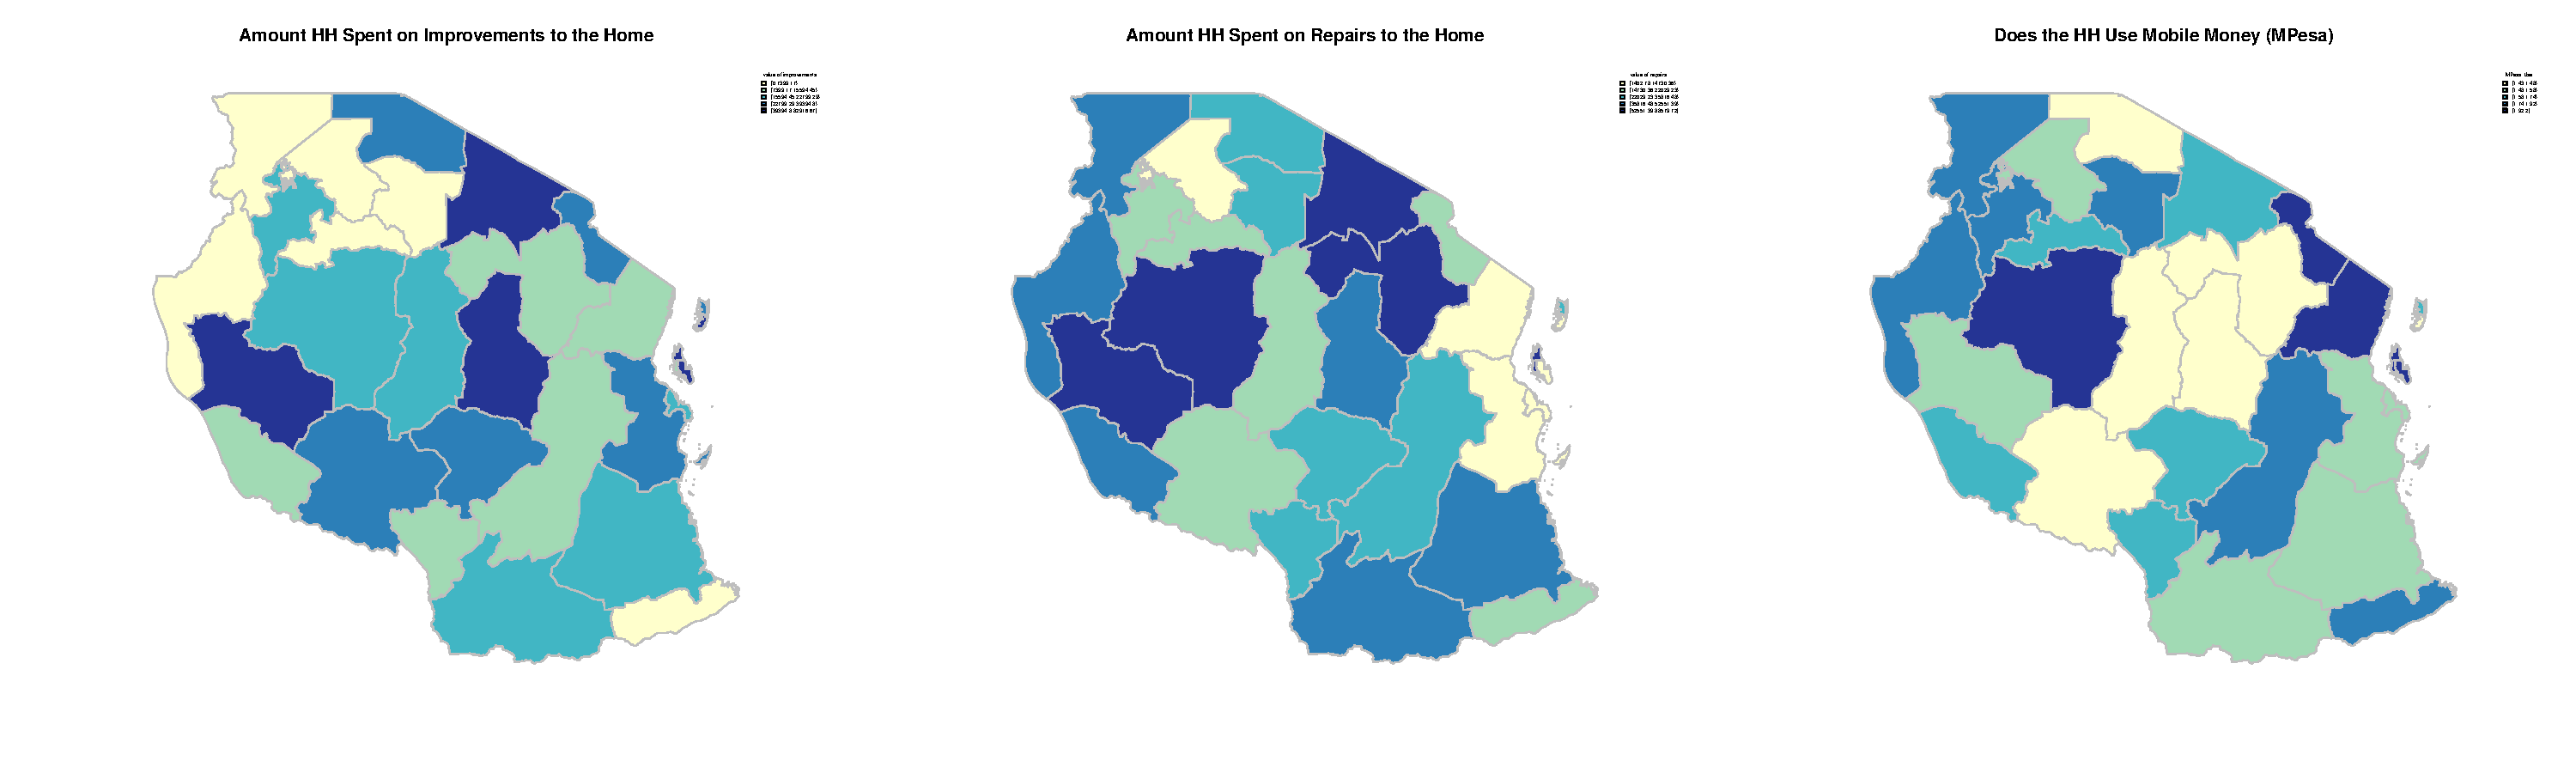
\includegraphics{PUBPOL599B_Final_Project_Exec-location}
\caption{Improvements to the Home, Repairs to the Home and Mobile Money Use by Region}
\end{figure}

\section{Conclusion}\

  These maps show that there is overlap among regions which spend a lot on improvements to the home, regions which spend a lot on repairs to the home, and regions which use mobile money. However, the relationships are not necessarily consistent. The converse can be observed as well. Therefore, the relationship between mobile money use and improvements to the home is inconclusive. 

  LSMS-ISA contains a wealth of information that could be harnessed to determine which factors influence whether an individual is willing and able to make improvements to his or her home. Additional work in this area could explore the relationship between advice from various sources (e.g. NGOs, etc.) and the value of improvements to the home, among other factors.  
  
\end{document}
